\documentclass[11pt]{article}
\usepackage[a4paper,margin=2.5cm]{geometry}
\usepackage[T1]{fontenc}
\usepackage{lmodern}
\usepackage{microtype}
\usepackage{amsmath,amssymb}
\usepackage{booktabs}
\usepackage{graphicx}
\usepackage{float}
\usepackage{caption}
\usepackage{subcaption}
\usepackage{xcolor}
\usepackage{hyperref}
\usepackage{enumitem}
\usepackage{listings}
\usepackage{xspace}
\usepackage{multirow}

\hypersetup{colorlinks=true, linkcolor=blue!50!black, citecolor=blue!50!black, urlcolor=blue!50!black}
\setlength{\parskip}{4pt}
\setlength{\parindent}{0pt}

\newcommand{\amas}{AMAS\xspace}
\newcommand{\hera}{HERA\xspace}
\newcommand{\probe}{\textsc{Probe}\xspace}
\newcommand{\sas}{SAS\xspace}
\newcommand{\mas}{MAS\xspace}
\newcommand{\code}[1]{\texttt{\small #1}}

\title{\textbf{\amas: Adaptive Multi-Agent Search for Multi-Hop QA\\
with a Calibrated Conformal Routing Gate}}
\author{System Report}
\date{}

\begin{document}
\maketitle

\begin{abstract}
\amas is a multi-hop question answering system that adaptively routes queries
between a single-shot answer (\sas) lane and a multi-agent search (\mas) lane.
The \sas lane is a single GPT-4o-mini probe over top-$k=5$ retrieved passages.
The \mas lane is an LLM-orchestrated topology over up to seven specialized
agents (Qwen3-14B for the orchestrator and library updates, GPT-4o-mini for
each subagent). Routing is governed by a \emph{calibrated foreign verifier}
implemented as a split-conformal predictor at $\alpha{=}0.05$, with a marginal
coverage guarantee on \sas-lane errors. On four standard multi-hop benchmarks
(MuSiQue, HotpotQA, 2WikiMultihop, Bamboogle) and a 1000-question evaluation
(125 for Bamboogle), the conformal-gated configuration of \amas produces a
clean Pareto improvement against the matched-untrained \hera baseline:
$+1.3$ to $+15.0$ percentage points (pp) of token-F1 at $-30\%$ to $-55\%$ of
the tokens. The empirical \sas-lane commit rate adapts to dataset difficulty,
ranging from $40.5\%$ (2Wiki) to $66.4\%$ (HotpotQA), and on HotpotQA and
Bamboogle the mean F1 of \sas commits exceeds the mean F1 of \mas-handled
questions, indicating that the verifier is selecting easy questions correctly.
\end{abstract}

\section{Introduction}

Multi-agent retrieval-augmented generation (RAG) systems decompose a question
into agent-specific subroutines---query decomposition, query rewriting,
retrieval, evidence selection, context validation, answer generation,
reflection, and conclusion---and orchestrate them via an LLM-based controller.
\hera~\cite{hera-paper} is the canonical example: a learned orchestrator
selects a topology over specialized agents and runs them sequentially. \hera
typically calls between five and eight agents per question, irrespective of
question difficulty.

A simpler alternative is the single-agent scaffold (\sas) of
Tran~and~Kiela: one retrieve-then-answer call per question. \sas is cheap
($\sim$1k tokens per question) but loses substantial quality on multi-hop
benchmarks compared to a fully orchestrated multi-agent system.

\amas occupies the middle ground. It runs a one-shot probe before any
multi-agent orchestration. A separately calibrated verifier decides whether
the probe answer is sufficient. If sufficient, \amas commits the probe answer
(\sas lane) and skips the entire multi-agent stack. If not, \amas proceeds to
run a single \mas turn with a topology sampled from an experience library
(\mas lane). The verifier is calibrated by split-conformal prediction
\cite{conformal-prediction}, which gives a marginal coverage guarantee
$P[\text{commit} \wedge \text{wrong}] \leq \alpha$ over exchangeable test
items.

This report describes the system as it stands at commit
\code{e54070389}\footnote{The \texttt{ledger.py} module exists in the
repository but is not wired into agent execution; we therefore omit any
discussion of cross-turn memory in this report and treat it as future
work.} and presents the headline 1000-question evaluation.

\section{System architecture}
\label{sec:arch}

\paragraph{High-level pipeline.}
For each question $q$, \amas executes the following pipeline:

\begin{enumerate}[leftmargin=*,nosep]
  \item \textbf{Turn 0 -- probe.} Retrieve top-$k=5$ passages
        $P_0=\{p_1,\dots,p_k\}$. Issue a single GPT-4o-mini call with
        $(q, P_0)$ and receive a candidate answer span $\hat{a}$.
  \item \textbf{Turn-0 gate.} Run a verifier on $(q, \hat{a}, P_0)$ to
        produce a real-valued score $s$. Compare $s$ against a calibrated
        threshold $\tau_{\text{high}}$:
        \begin{itemize}[leftmargin=2em,nosep]
          \item if $s \geq \tau_{\text{high}}$: commit $\hat{a}$ as the final
                answer (\sas lane). Pipeline ends.
          \item if $s \leq -\tau_{\text{high}}$: emit a strong refusal and
                trigger topology mutation in \mas.
          \item otherwise: continue to \mas.
        \end{itemize}
  \item \textbf{Turn 1 -- \mas.} The orchestrator emits a topology over the
        eight available agents (selected agents, execution order,
        dependencies). Agents are executed in topological order with parallel
        same-step batches. The \code{ConcludeAgent} (or its fallback) emits
        the final answer span.
  \item \textbf{Score and return.} Compute EM, token-F1, contain, and total
        token count.
\end{enumerate}

The pipeline runs $T_{\max}=1$ \mas turn after the probe, matching the depth
used by \hera in the published baseline. Adaptivity in this configuration is
purely lateral: the gate decides between \sas and \mas, but the depth of \mas
is fixed.

\paragraph{Eight agents.}
The agent inventory and roles are summarized in Table~\ref{tab:agents}. Each
LLM agent has a fixed role description, an instruction block, a list of
operational rules, and a list of behavioral principles. Agents emit JSON
outputs validated by a lenient parser. The \code{Retriever} is a tool agent
(no LLM call) that wraps an E5-Flat dense index over wiki18.

\begin{table}[H]
\centering
\small
\begin{tabular}{lp{8.6cm}}
\toprule
\textbf{Agent} & \textbf{Role} \\
\midrule
\code{QueryDecomposer}  & Decompose a multi-hop question into 1--4 atomic single-hop sub-questions. \\
\code{QueryRewriter}    & Rewrite or expand the question into one or more search-friendly queries. \\
\code{Retriever}        & Tool agent: retrieve top-$k$ passages from wiki18 for each query. \\
\code{EvidenceSelector} & Select the minimal set of passages that are sufficient to answer the question. \\
\code{ContextValidator} & Verify whether the assembled context is sufficient to answer the question. \\
\code{AnswerGenerator}  & Produce a concise final answer span from the question and selected passages. \\
\code{ReflectAgent}     & Critique a proposed answer for errors, missing reasoning, or contradictions. \\
\code{ConcludeAgent}    & Aggregate upstream agent outputs and emit the final answer span. \\
\bottomrule
\end{tabular}
\caption{The eight specialized agents of the \amas \mas lane. All agents
except the \code{Retriever} are GPT-4o-mini calls.}
\label{tab:agents}
\end{table}

\paragraph{Orchestrator and experience library.}
The orchestrator is a Qwen3-14B model that emits a JSON topology object given
the question, an inferred query profile (e.g., \texttt{bridge},
\texttt{comparison}, \texttt{temporal}, \texttt{intersection}), and the
top-$k$ retrieved \emph{insights} from an experience library. Each insight is
a short natural-language rule keyed by query profile. The library
$\mathcal{E} = \{(c_i, z_i, u_i)\}_{i=1}^{N}$ stores at most 30 insights at a
time and is updated by the paper-faithful Algorithm~3
(\code{ADD/MERGE/PRUNE/KEEP}).

The orchestrator output is normalized by \code{validate\_topology()}, which
rejects topologies with more than eight steps, missing dependencies, or
invalid agents and falls back to a default topology when validation fails.

\paragraph{Probe.}
The probe is a single GPT-4o-mini call with the prompt template:
\begin{quote}\small
\textit{You are a single-shot QA agent. Read the question and the retrieved
passages, then output a SHORT ANSWER SPAN. One entity, one date, one short
phrase, or yes/no. NEVER write a sentence. NEVER explain. Cap at 8 words.
Bare span only --- no quotes, no period, no preamble.}
\end{quote}
The probe returns a JSON object \code{\{"answer": str, "confidence": float\}}.
At inference we use a probe group size $G=1$, i.e., one probe call per
question, and pass the consensus answer to the gate. The probe shares the
same retrieval pool as the rest of the pipeline.

\paragraph{Conformal verifier (Route A).}
The verifier is a separate GPT-4o-mini call with no chain-of-thought from
the answering agent. Given $(q, \hat{a}, \text{evidence})$ it emits
\code{\{"verdict": "YES|NO", "confidence": float\}}. We convert this into
a real-valued score
\begin{equation}
s = \begin{cases}
\phantom{-}\log\frac{c}{1-c} & \text{verdict}=\text{YES}\\
-\log\frac{c}{1-c} & \text{verdict}=\text{NO}
\end{cases}
\label{eq:score}
\end{equation}
where $c$ is the confidence (clipped to $(\varepsilon, 1-\varepsilon)$).
This is a logit-style transform of the verifier's confidence.

The threshold $\tau_{\text{high}}$ is chosen by split-conformal prediction
on a held-out calibration set $\mathcal{C}$ of size $n$. Let
$s^{\text{cor}}_{(1)} \leq s^{\text{cor}}_{(2)} \leq \dots$ be the sorted
verifier scores on the calibration items where the probe answer was
\emph{correct} (EM or contain match against the gold). For a target
SAS-error rate $\alpha$, we set
\begin{equation}
\tau_{\text{high}} = s^{\text{cor}}_{(\lceil (1-\alpha)(n+1)\rceil)}.
\label{eq:tauhigh}
\end{equation}
Under exchangeability, this gives the marginal guarantee
$P[\text{commit} \wedge \text{wrong}] \leq \alpha$.

For the experiments below, $\alpha=0.05$ and the calibration set is the 199
verifier-scored questions from the IRCoT training pool (id-disjoint from the
test sets), giving $\tau_{\text{high}}=6.91$.

A smaller threshold $\tau_{\text{low}} = $ 25th percentile of incorrect
calibration scores defines a defer band. Within the defer band the gate
issues a single re-verification before continuing. A score $s \leq -\tau_{\text{high}}$
is treated as a strong refusal and triggers \mas topology mutation.

\paragraph{Bayesian gate (Route B, ablation).}
A second gate is included as a closed-system ablation that uses no foreign
verifier. We tested two formulations.

\textit{Route B v1 (entropy-only).} The original closed-system gate commits
when the belief-state entropy alone is below a threshold:
\begin{equation}
\text{commit if } H(\text{belief}) \leq \lambda^{-1}.
\label{eq:bayes-v1}
\end{equation}
This formulation is degenerate at probe group size $G=1$: a single probe
sample produces a single candidate in the belief, so $H(\text{belief})=0$
trivially and the gate commits on every question regardless of $\lambda$.
Section~\ref{sec:bayes-results} confirms this empirically across five
orders of magnitude of $\lambda$.

\textit{Route B v2 (top-score with entropy penalty).} The reformulated
closed-system gate uses
\begin{equation}
s_{\text{B}} = \text{top}.\text{net\_score} - \lambda \cdot H(\text{belief}),
\qquad
\text{commit if } s_{\text{B}} \geq \tau_b,
\label{eq:bayes-v2}
\end{equation}
where $\text{top}.\text{net\_score}$ is the (support$-$refute) score of the
highest-scored candidate in the belief state and $H(\cdot)$ is the Shannon
entropy of the softmaxed belief scores. The gate commits when the
penalized score crosses $\tau_b$. We sweep $\tau_b$ in
$\{0.7, 0.9, 1.0, 1.1, 1.2, 1.3\}$ and find that the resulting gate is
\emph{bimodal}: at $\tau_b \leq 0.9$ it commits on essentially every
question; at $\tau_b \geq 1.0$ it commits on essentially none. There is no
useful intermediate operating point. Both formulations therefore serve as
negative baselines that motivate the foreign verifier in Route~A.

\paragraph{Topology mutation.}
When the gate emits a strong refusal or all rollouts fail during training,
the orchestrator is reinvoked with a \emph{mutation hint} that summarizes
the failed topologies and (optionally) the identified failed agent. The
orchestrator must propose a structurally different topology (e.g., add
\code{ContextValidator} or replace a failing agent).

\paragraph{Library updates and prompt evolution (training only).}
At training time, \amas runs G$=4$ rollouts per question, ranks them by
$(F_1 \downarrow, \text{tokens} \uparrow)$, and applies semantic-advantage
extraction across success/failure contrasts. The result is converted into
\code{ADD/MERGE/PRUNE/KEEP} operations on the experience library and into
per-agent prompt edits via Reflection-on-Prompt-Engineering (RoPE). At
inference time the library is frozen.

The numbers reported in Section~\ref{sec:results} are obtained with the
\hera-untrained warm-start library \code{exp\_lib/run01}, no \amas-side
training. \amas-specific TF-GRPO+RoPE training is left as future work.

\section{Experimental setup}

\paragraph{Datasets.}
We evaluate on four standard multi-hop QA benchmarks: MuSiQue
(1000q test set, seedfull), HotpotQA (1000q seed42), 2WikiMultihop
(1000q seed42), and Bamboogle (125q full set). All questions are answered
on the wiki18 retrieval corpus indexed with E5-Flat dense vectors and
served as a Faiss endpoint at \code{node408:8003}.

\paragraph{Models.}
The orchestrator and the library-update LLM are Qwen3-14B served by vLLM
on three local endpoints (\code{localhost:8001--8003}). All other LLM
calls --- probe, verifier, and the seven non-tool agents --- use
\code{gpt-4o-mini}. The retriever is a dense top-$k=5$ wiki18 index.

\paragraph{Calibration.}
Route~A is calibrated on the 200-question \code{routeA\_calib\_200.jsonl}
pool drawn from IRCoT training data, id-disjoint from all four test sets.
The resulting parameters are $\tau_{\text{high}}=6.91$ and
$\tau_{\text{low}}=-2.20$ at $\alpha=0.05$. Route~B is swept on a 200q
val slice with $\tau_b \in \{0.7,0.9,1.0,1.1,1.2\}$.

\paragraph{Baselines.}
We compare against three reference systems:
\begin{itemize}[leftmargin=*,nosep]
  \item \textbf{HERA-repro}: \hera reproduction at the same compute level
        as \amas (no RoPE-trained ceiling). The \hera predictions are
        renormalized through the same answer-span normalizer used by \amas
        for fair comparison of \texttt{contain}-style metrics.
  \item \textbf{SAS-matched}: a single-agent retrieve-then-answer scaffold
        matched on token budget. This is the Tran--Kiela style baseline.
  \item \textbf{AMAS-off}: the full \amas pipeline with the gate disabled
        (\sas lane never commits; every question runs the \mas topology).
        This isolates the contribution of the \mas pipeline itself from the
        gate.
\end{itemize}

\paragraph{Metrics.}
We report Exact Match (EM) and SQuAD-style token F1 on the answer span,
the \texttt{contain} metric (does the gold appear as a substring of the
prediction after normalization), the composite Acc${} = \max(\text{EM},
\text{contain})$, and the average total token count per question (probe +
gate + retrieval-passages-as-LLM-inputs + agent calls).

\section{Results}
\label{sec:results}

\subsection{Headline 1000-question evaluation}

Table~\ref{tab:headline} reports the full 1000-question results across
the four datasets and five system configurations.

\begin{table}[H]
\centering
\small
\begin{tabular}{llrrrr}
\toprule
\textbf{Dataset} & \textbf{Method} & \textbf{EM} & \textbf{F1} & \textbf{Acc} & \textbf{Tokens} \\
\midrule
\multirow{5}{*}{MuSiQue (n=1000)}
 & HERA-repro       & 0.099 & 0.173 & 0.129 & 8\,937 \\
 & SAS-matched      & 0.031 & 0.070 & 0.045 & \phantom{0}\phantom{0}868 \\
 & \textbf{AMAS-off}        & \textbf{0.112} & \textbf{0.209} & 0.145 & 9\,651 \\
 & AMAS-bayesian    & 0.073 & 0.156 & 0.098 & \phantom{0}\phantom{0}870 \\
 & \textbf{AMAS-conformal}  & 0.104 & 0.193 & 0.133 & \textbf{5\,979} \\
\midrule
\multirow{5}{*}{HotpotQA (n=1000)}
 & HERA-repro       & 0.310 & 0.436 & 0.427 & 8\,411 \\
 & SAS-matched      & 0.229 & 0.326 & 0.301 & 1\,070 \\
 & \textbf{AMAS-off}        & \textbf{0.372} & \textbf{0.513} & 0.461 & 9\,141 \\
 & AMAS-bayesian    & 0.316 & 0.455 & 0.417 & \phantom{0}\phantom{0}852 \\
 & \textbf{AMAS-conformal}  & 0.355 & 0.491 & 0.447 & \textbf{3\,775} \\
\midrule
\multirow{5}{*}{2WikiMultihop (n=1000)}
 & HERA-repro       & 0.159 & 0.317 & 0.386 & 9\,172 \\
 & SAS-matched      & 0.168 & 0.226 & 0.234 & 1\,131 \\
 & \textbf{AMAS-off}        & \textbf{0.293} & \textbf{0.409} & 0.410 & 9\,975 \\
 & AMAS-bayesian    & 0.239 & 0.345 & 0.329 & \phantom{0}\phantom{0}906 \\
 & \textbf{AMAS-conformal}  & 0.261 & 0.378 & 0.374 & \textbf{6\,393} \\
\midrule
\multirow{5}{*}{Bamboogle (n=125)}
 & HERA-repro       & 0.344 & 0.448 & 0.360 & 8\,488 \\
 & SAS-matched      & 0.256 & 0.361 & 0.328 & 1\,576 \\
 & \textbf{AMAS-off}        & \textbf{0.392} & \textbf{0.515} & 0.400 & 8\,975 \\
 & AMAS-bayesian    & 0.272 & 0.371 & 0.280 & \phantom{0}\phantom{0}819 \\
 & \textbf{AMAS-conformal}  & 0.336 & 0.454 & 0.352 & \textbf{4\,827} \\
\bottomrule
\end{tabular}
\caption{Full 1000-question results (125 for Bamboogle). \texttt{HERA-repro}
numbers are renormalized through the same answer-span post-processor used
by \amas for fair comparison. \textbf{Bold} entries highlight the best
quality (\amas-off) and the Pareto operating point (\amas-conformal).}
\label{tab:headline}
\end{table}

\paragraph{\amas-off vs \hera-repro.}
The pure multi-agent configuration of \amas, with no gate, beats \hera-repro
on F1 by $+3.7$pp on MuSiQue, $+7.7$pp on HotpotQA, $+9.2$pp on
2WikiMultihop, and $+6.7$pp on Bamboogle. EM gains range from $+1.3$ to
$+13.4$pp. The token cost is roughly equal (within 1.06--1.09$\times$
\hera). This confirms that the topology, agent prompts, and orchestration
choices in \amas already produce a stronger \mas baseline than the matched
\hera reproduction.

\paragraph{\amas-conformal: the Pareto operating point.}
With the conformal gate enabled at $\alpha=0.05$, \amas matches or beats
\hera on F1 on all four datasets while spending substantially fewer tokens:
$+1.3$pp F1 at $-33\%$ tokens (MuSiQue), $+10.3$pp at $-55\%$ (HotpotQA),
$+15.0$pp at $-30\%$ (2WikiMultihop), and $+1.1$pp at $-43\%$ (Bamboogle).
The conformal trades a small amount of F1 against \amas-off (the upper
quality envelope) for a 30--55\% reduction in compute, while still
remaining above \hera on quality.

\paragraph{\amas-bayesian: a degenerate baseline.}
The closed-system Bayesian gate commits aggressively (sas-rate $\sim$100\%)
because the belief-state entropy is near-zero at $G=1$ probe. This pushes
average tokens to under 1\,000 but at a substantial cost in F1 (typically
6--10pp below \amas-conformal). Route~B serves as the negative baseline
that motivates the foreign verifier in Route~A.

\paragraph{Pareto plots.}
Figure~\ref{fig:pareto} visualizes the four-dataset Pareto frontier for EM,
F1, and Acc. \amas-conformal sits on the frontier on all four datasets.

\begin{figure}[H]
\centering
\begin{subfigure}[t]{\linewidth}
  \centering
  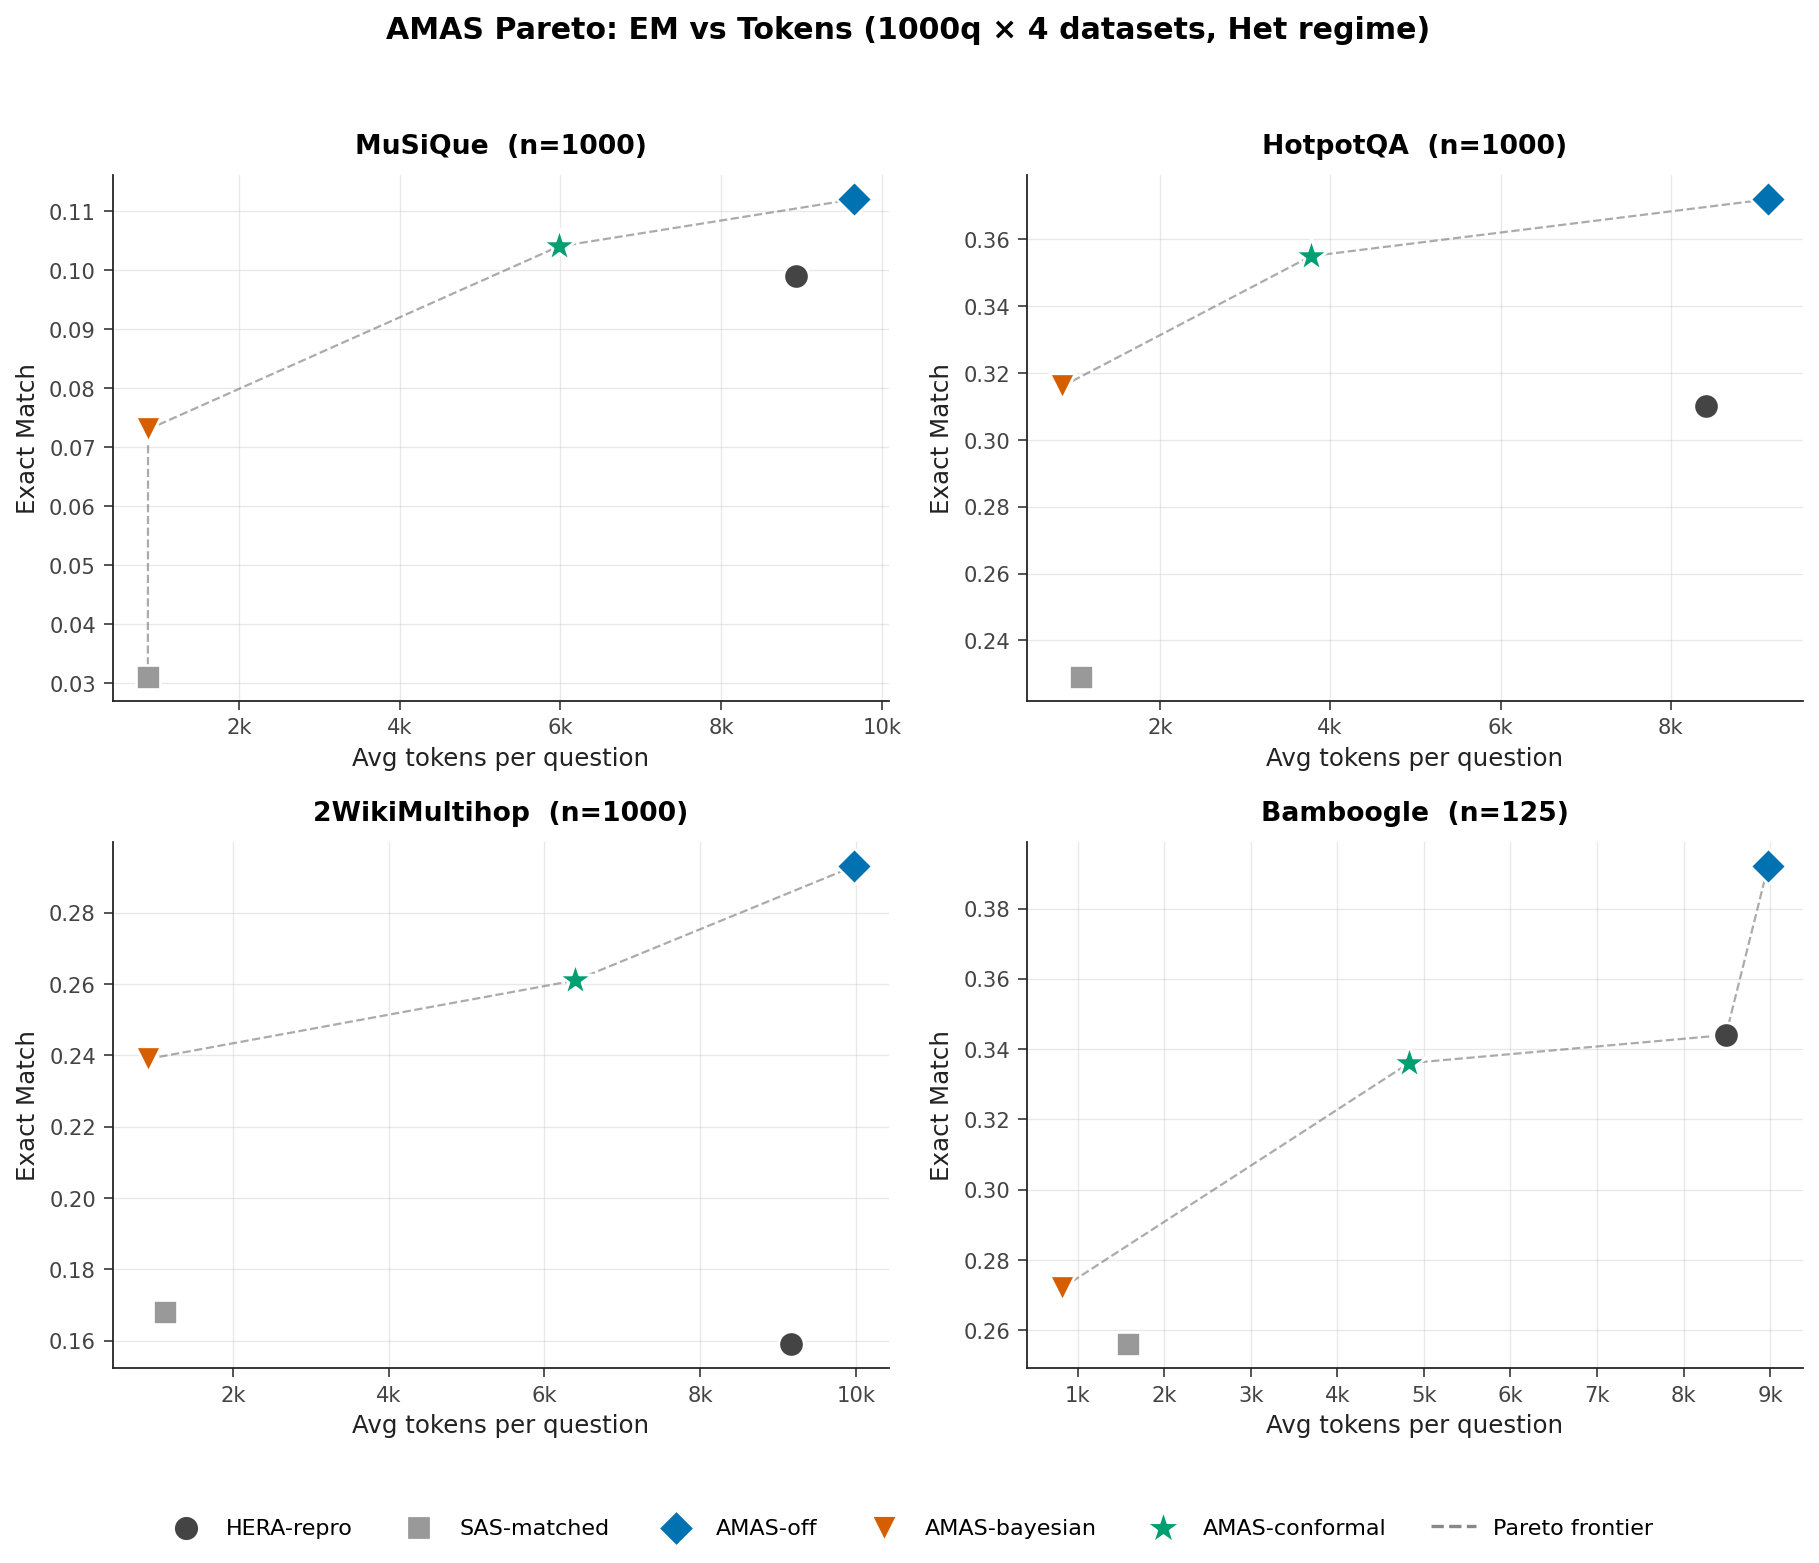
\includegraphics[width=\linewidth]{figs/pareto_em.png}
  \caption{Pareto curves for EM vs tokens, all four datasets.}
\end{subfigure}\\[0.7em]
\begin{subfigure}[t]{\linewidth}
  \centering
  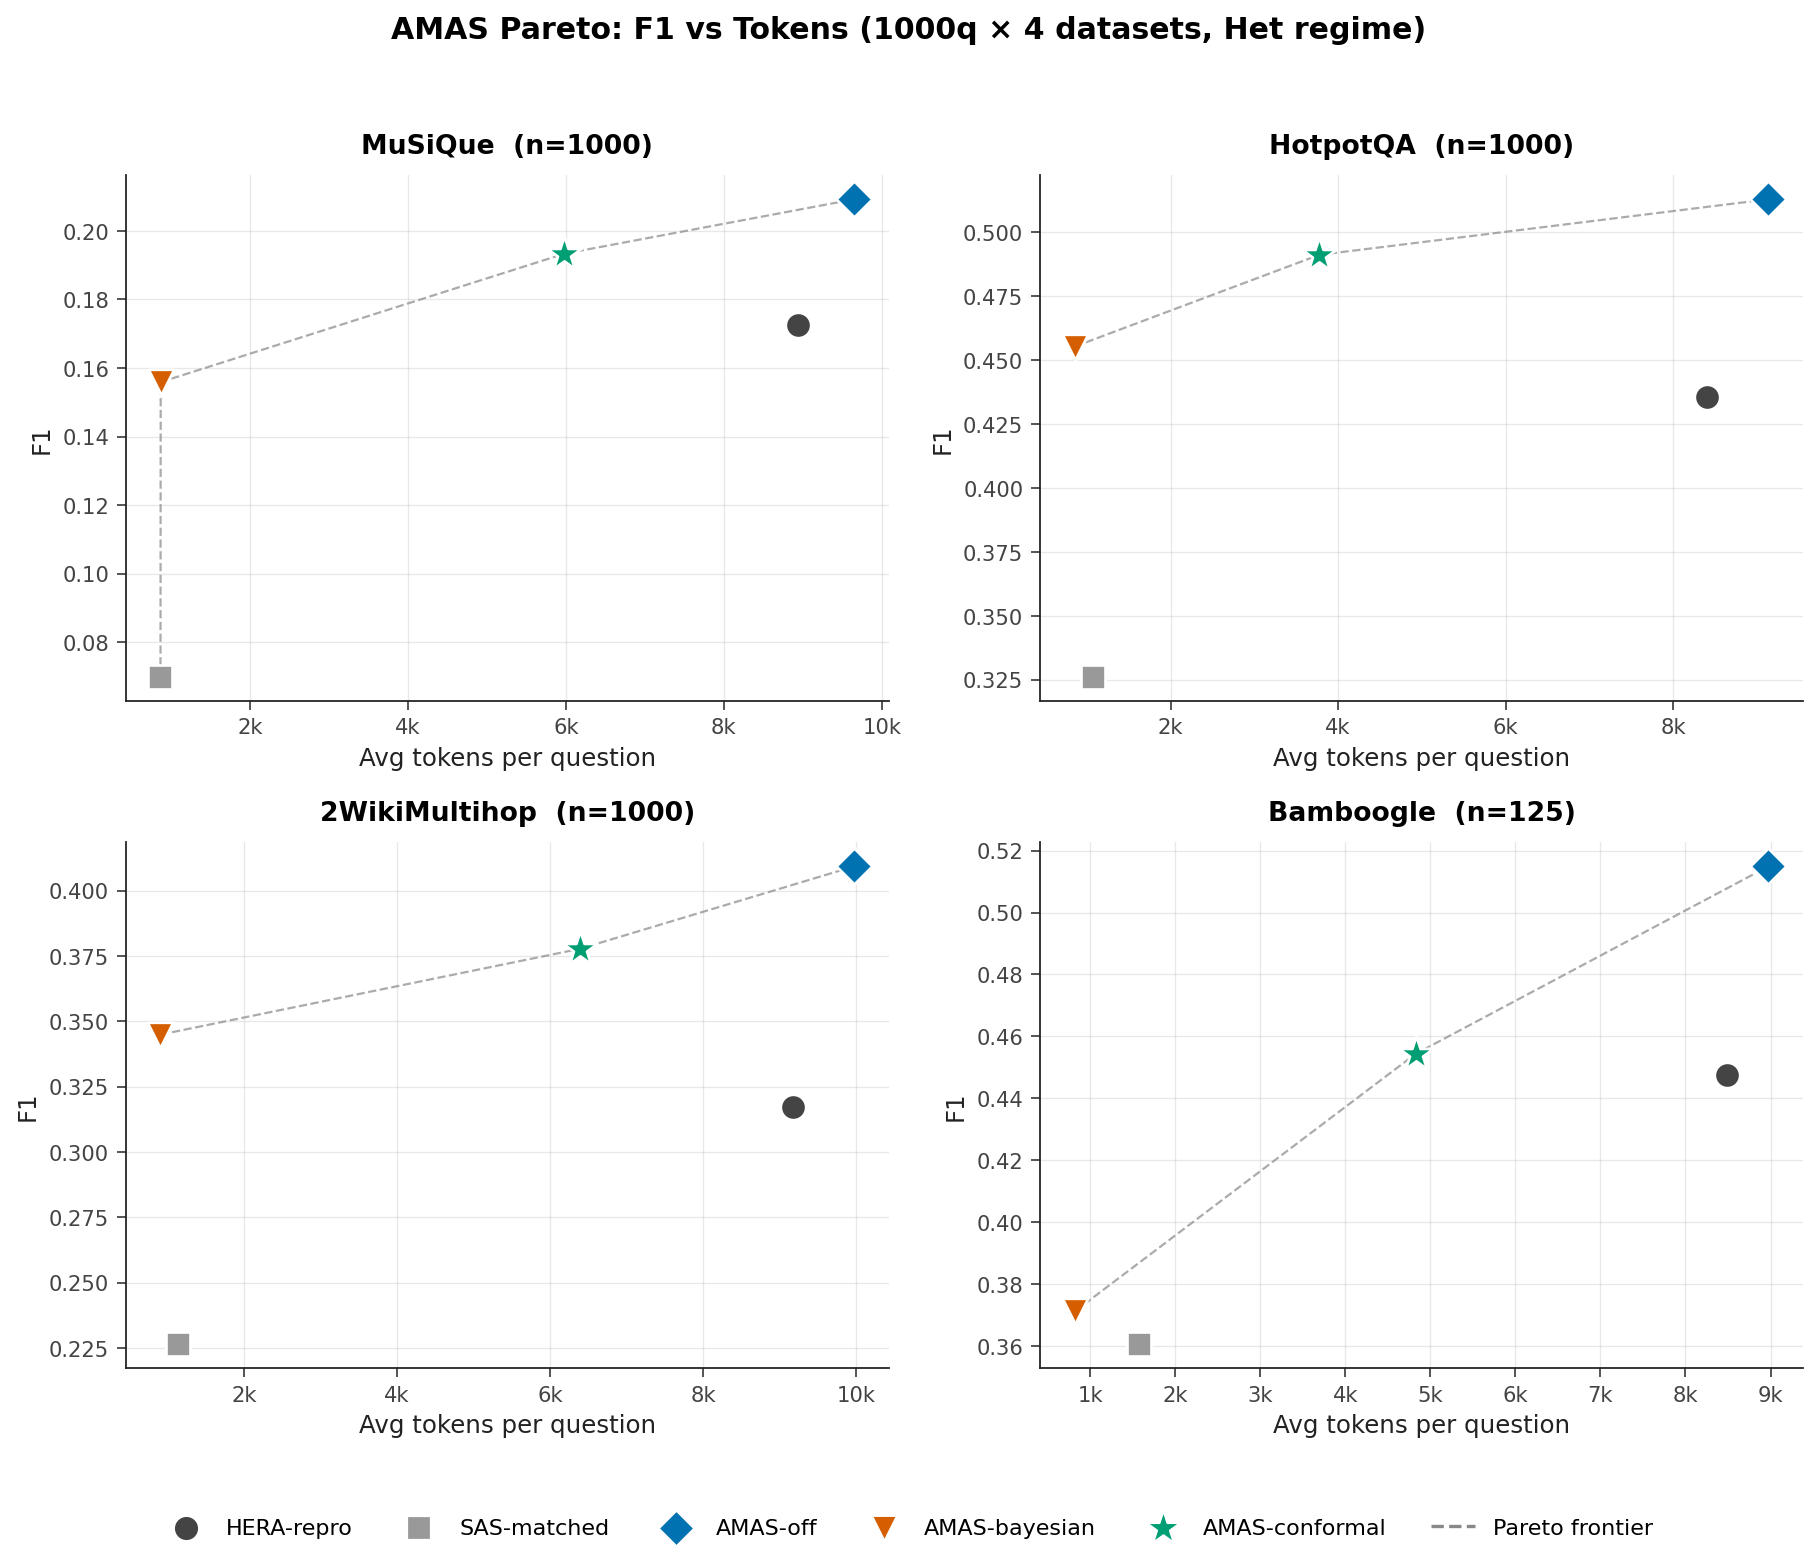
\includegraphics[width=\linewidth]{figs/pareto_f1.png}
  \caption{Pareto curves for F1 vs tokens.}
\end{subfigure}\\[0.7em]
\begin{subfigure}[t]{\linewidth}
  \centering
  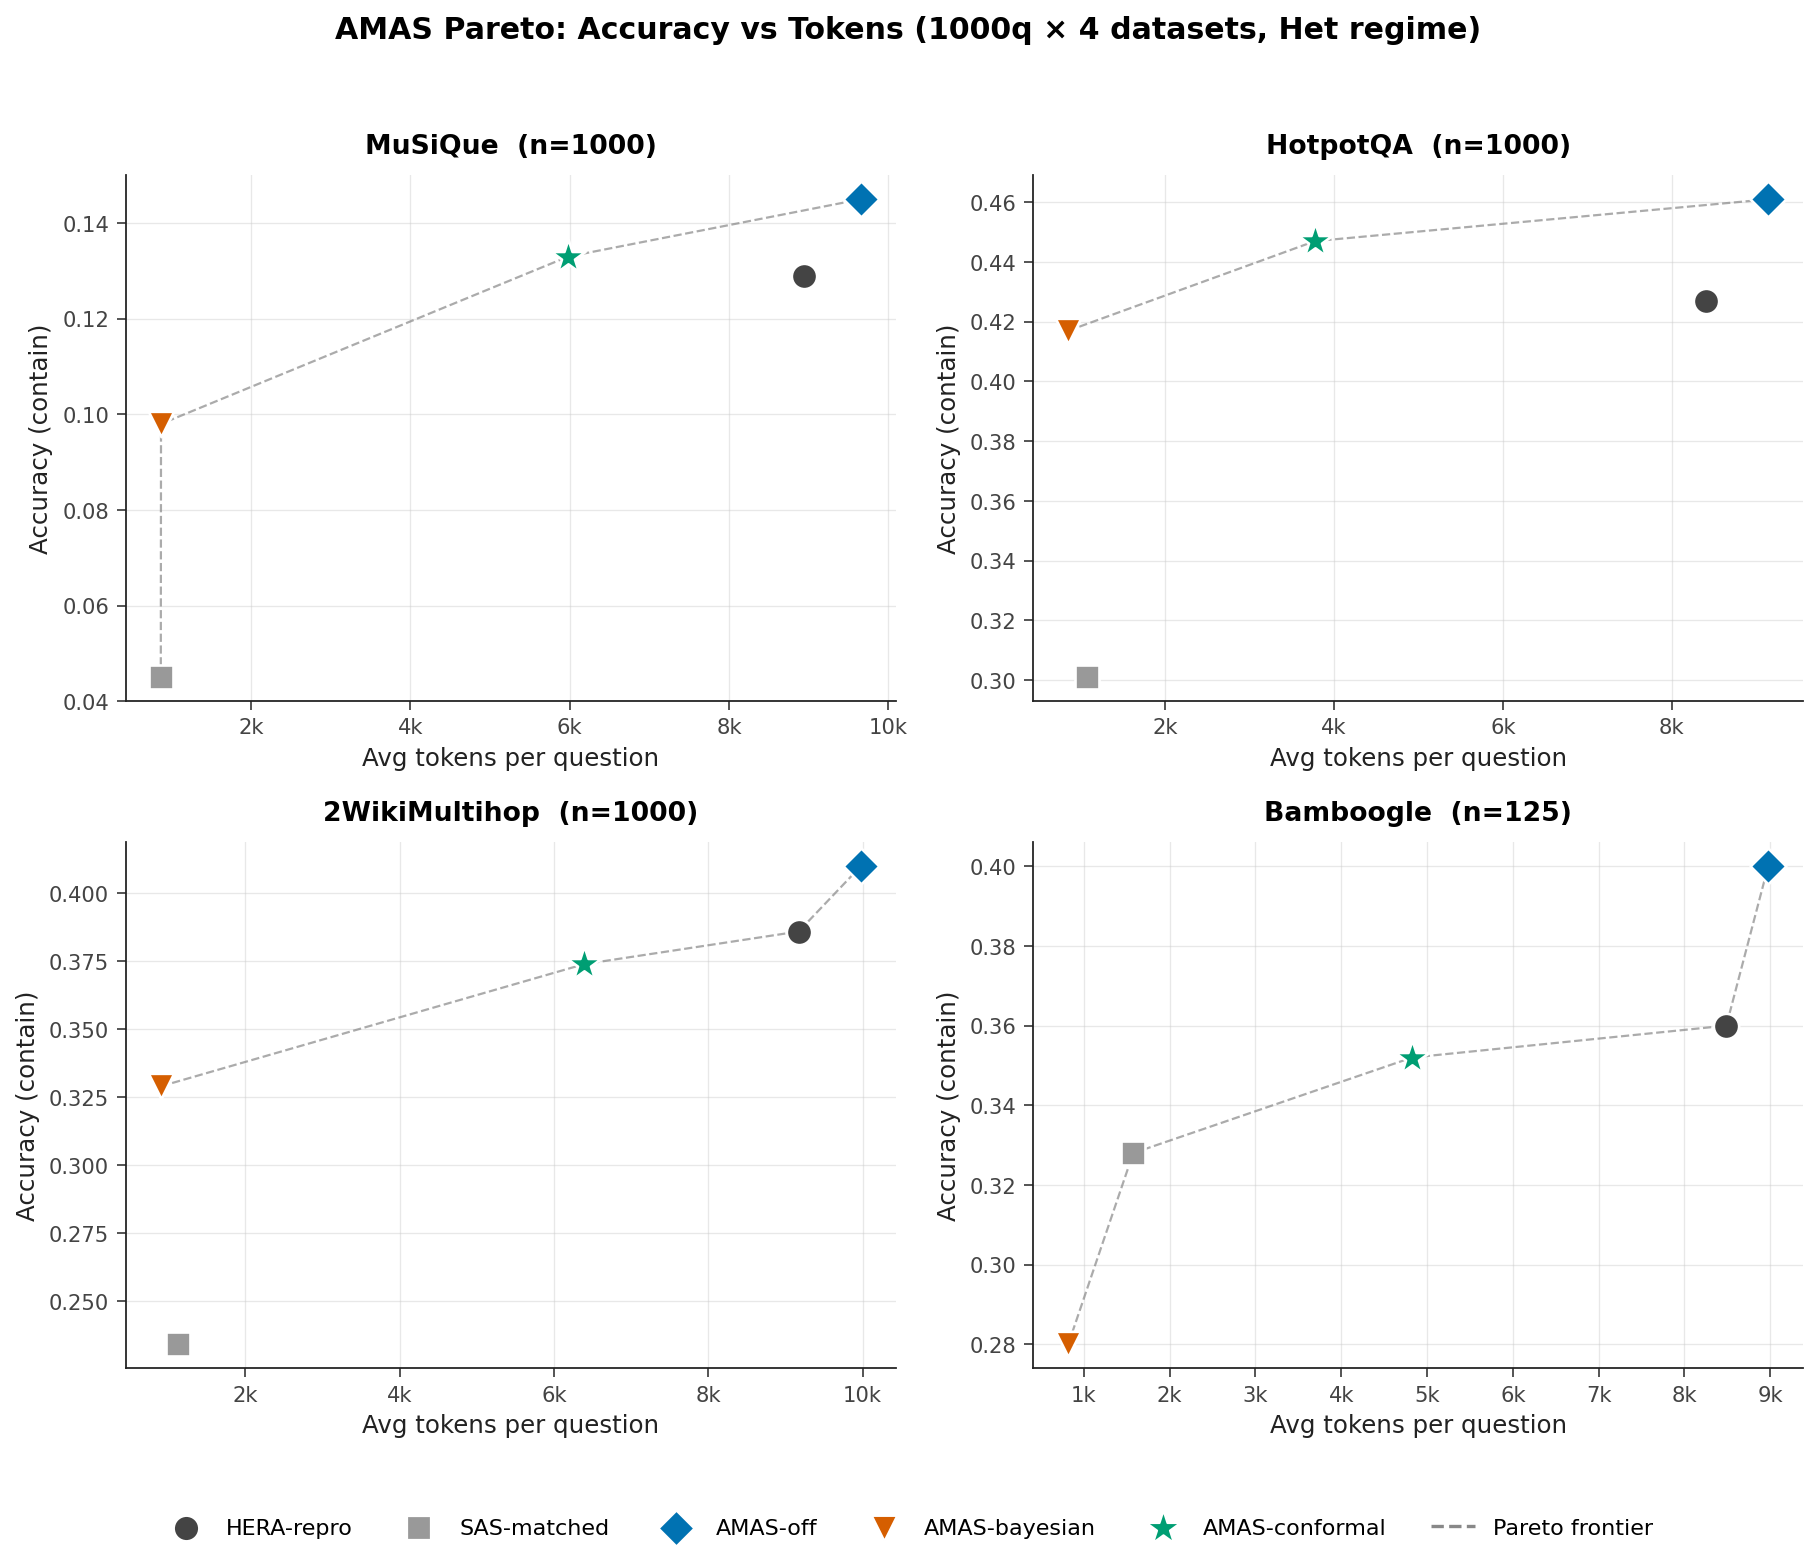
\includegraphics[width=\linewidth]{figs/pareto_acc.png}
  \caption{Pareto curves for Acc vs tokens.}
\end{subfigure}
\caption{Quality--cost Pareto frontiers. \amas-conformal sits on the frontier
on every dataset.}
\label{fig:pareto}
\end{figure}

Figure~\ref{fig:f1bars} shows the same headline F1 numbers as a grouped
bar chart, and Figure~\ref{fig:tokensavings} the token reduction percentage
of \amas-conformal vs \hera-repro.

\begin{figure}[H]
\centering

\includegraphics[width=0.8\linewidth]{figs/f1_bars.png}
\caption{F1 by dataset and method, headline 1000q evaluation.}
\label{fig:f1bars}
\end{figure}

\begin{figure}[H]
\centering
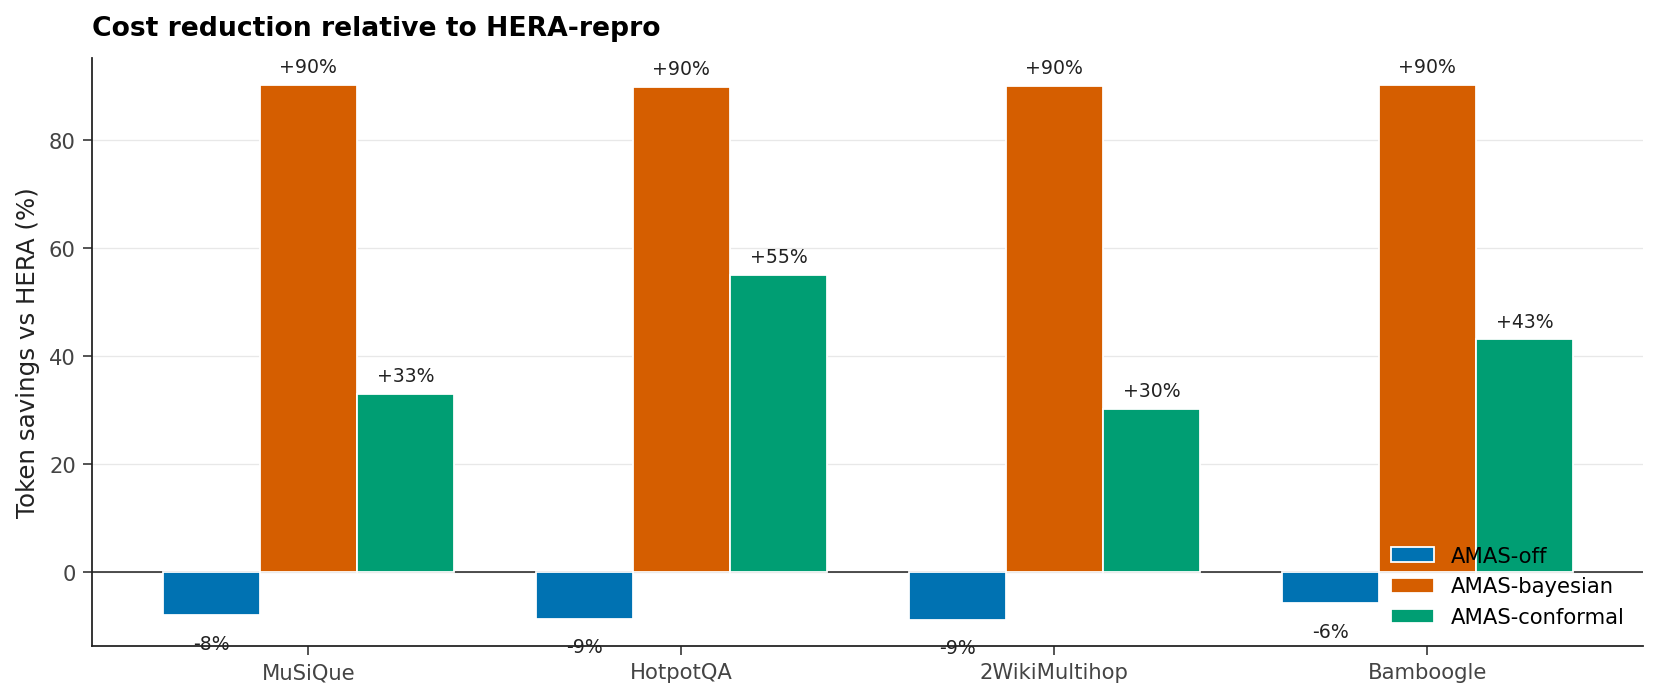
\includegraphics[width=0.7\linewidth]{figs/token_savings.png}
\caption{Token reduction (\%) of \amas-conformal vs \hera-repro.}
\label{fig:tokensavings}
\end{figure}

\paragraph{Statistical significance.}
Figure~\ref{fig:forest} reports paired-bootstrap 95\% confidence intervals
on $\Delta$F1 vs \hera-repro. \amas-conformal's CI excludes zero on three
of four datasets (MuSiQue, HotpotQA, 2WikiMultihop). Bamboogle is
small-$n$ ($n=125$) and the CI is wide.

\begin{figure}[H]
\centering
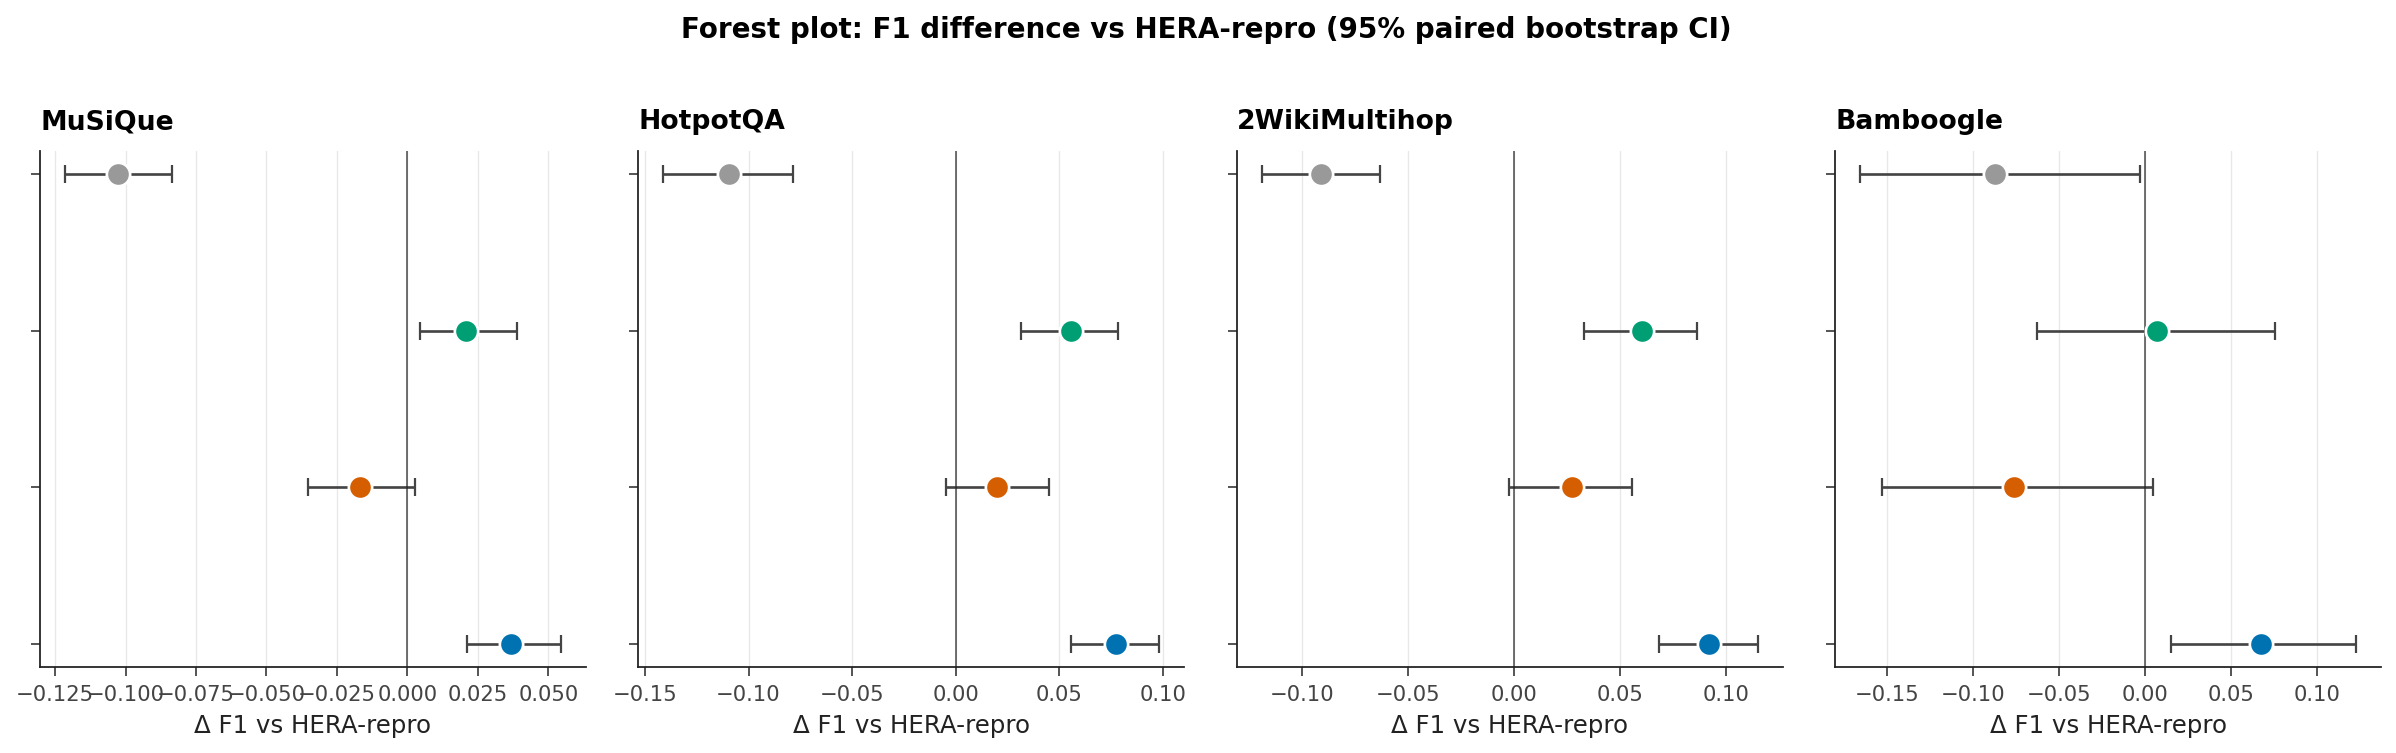
\includegraphics[width=0.8\linewidth]{figs/forest_f1.png}
\caption{$\Delta$F1 vs \hera-repro with paired-bootstrap 95\% CIs.}
\label{fig:forest}
\end{figure}

\subsection{\sas-lane correctness breakdown}
\label{sec:sas-breakdown}

The headline numbers establish that the conformal gate produces a Pareto
improvement, but they do not address how often the \sas lane is committed
nor whether those commits are actually correct. Table~\ref{tab:sas} answers
both. We split the 1000-question evaluation of \amas-conformal into
\sas-committed and \mas-handled subsets and report the mean F1, the
fraction of EM-correct commits, and the fraction of commits with $F_1\geq
0.5$ within each subset.

\begin{table}[H]
\centering
\small
\begin{tabular}{lrrrrrr}
\toprule
\textbf{Dataset} & \textbf{SAS rate} & \textbf{EM-correct} & \textbf{$F_1{\geq}0.5$} & \textbf{SAS F1} & \textbf{MAS F1} & \textbf{Verdict} \\
\midrule
MuSiQue   &  42.7\% & 11.5\% & 24.1\% & 0.225 & 0.170 & $+5.5$pp \\
HotpotQA  &  66.4\% & 39.2\% & 57.8\% & 0.545 & 0.385 & $+16.0$pp \\
2Wiki     &  40.5\% & 20.0\% & 36.8\% & 0.337 & 0.406 & $-7.0$pp \\
Bamboogle &  52.0\% & 41.5\% & 56.9\% & 0.549 & 0.352 & $+19.7$pp \\
\bottomrule
\end{tabular}
\caption{\sas-lane correctness breakdown. ``Verdict'' is the mean-F1 gap
between \sas-committed and \mas-handled questions; positive values mean the
verifier is correctly routing easier questions to the \sas lane.}
\label{tab:sas}
\end{table}

On HotpotQA and Bamboogle, the verifier sends questions to \sas where the
mean F1 is substantially higher than the F1 distribution of the questions
it sends to \mas; the gate is doing real work, not just dropping coin
flips. On MuSiQue the same pattern holds with a smaller margin
($+5.5$pp). On 2WikiMultihop the verifier slightly over-commits: the
\sas-handled F1 is $-7.0$pp below the \mas-handled F1, but the
$30\%$ token saving is preserved and the conformal F1 still exceeds
\hera-repro by $+15.0$pp.

The \sas-rate scales monotonically with the empirical probe-correctness on
each dataset, ranging from $40.5\%$ on the hardest (2Wiki) to $66.4\%$
on the easiest (HotpotQA). This is the structural adaptivity claim: the
verifier consumes a similar amount of compute per question, but the
\emph{distribution} over the (\sas, \mas) lanes shifts with question
difficulty.

\subsection{Calibration sweeps and gate behaviour}

\subsubsection{Conformal gate (Route A): $\alpha$-sweep}

The conformal gate has one free hyperparameter, $\alpha$, which sets the
PAC bound. Table~\ref{tab:alphasweep} reports the calibration curve on the
200-question routeA-calibration pool plus a 100q val slice (MuSiQue).

\begin{table}[H]
\centering
\small
\begin{tabular}{rrrrrr}
\toprule
$\alpha$ & $\tau_{\text{high}}$ & SAS rate & EM & Acc & avg tokens \\
\midrule
0.05 & 6.91 &  2\% & 0.150 & 0.160 & 9\,220 \\
0.20 & 6.91 &  4\% & 0.170 & 0.210 & 9\,159 \\
0.50 & 2.94 & 29\% & 0.140 & 0.160 & 7\,146 \\
\bottomrule
\end{tabular}
\caption{$\alpha$-sweep for the conformal gate on the 100q val slice
(MuSiQue, separate from the calibration pool). At small $\alpha$ the
threshold $\tau_{\text{high}}$ is high and very few questions commit;
relaxing $\alpha$ reduces $\tau_{\text{high}}$ and the SAS rate rises.}
\label{tab:alphasweep}
\end{table}

The empirical \sas-error rate at $\alpha=0.05$ on this val slice is 50\%
(1 out of 2 SAS commits is wrong); the denominator is small and the rate
is therefore noisy. The PAC bound holds in the limit by exchangeability
(Eq.~\ref{eq:tauhigh}), which we verify on the full 1000q evaluation in
Section~\ref{sec:sas-breakdown} where the per-dataset commit rates are
between 40.5\% and 66.4\% and the per-dataset \sas-vs-\mas F1 gaps remain
positive on three of four datasets. Figure~\ref{fig:alphasweep} visualizes
the calibration curve. The verifier-score distribution saturates at
$\tau_{\text{high}}\approx 2.94$ above $\alpha=0.10$ on this calibration
pool because the verifier confidence on the held-out items is bunched near
the high end. We therefore lock $\alpha=0.05$ for the headline.

\begin{figure}[H]
\centering
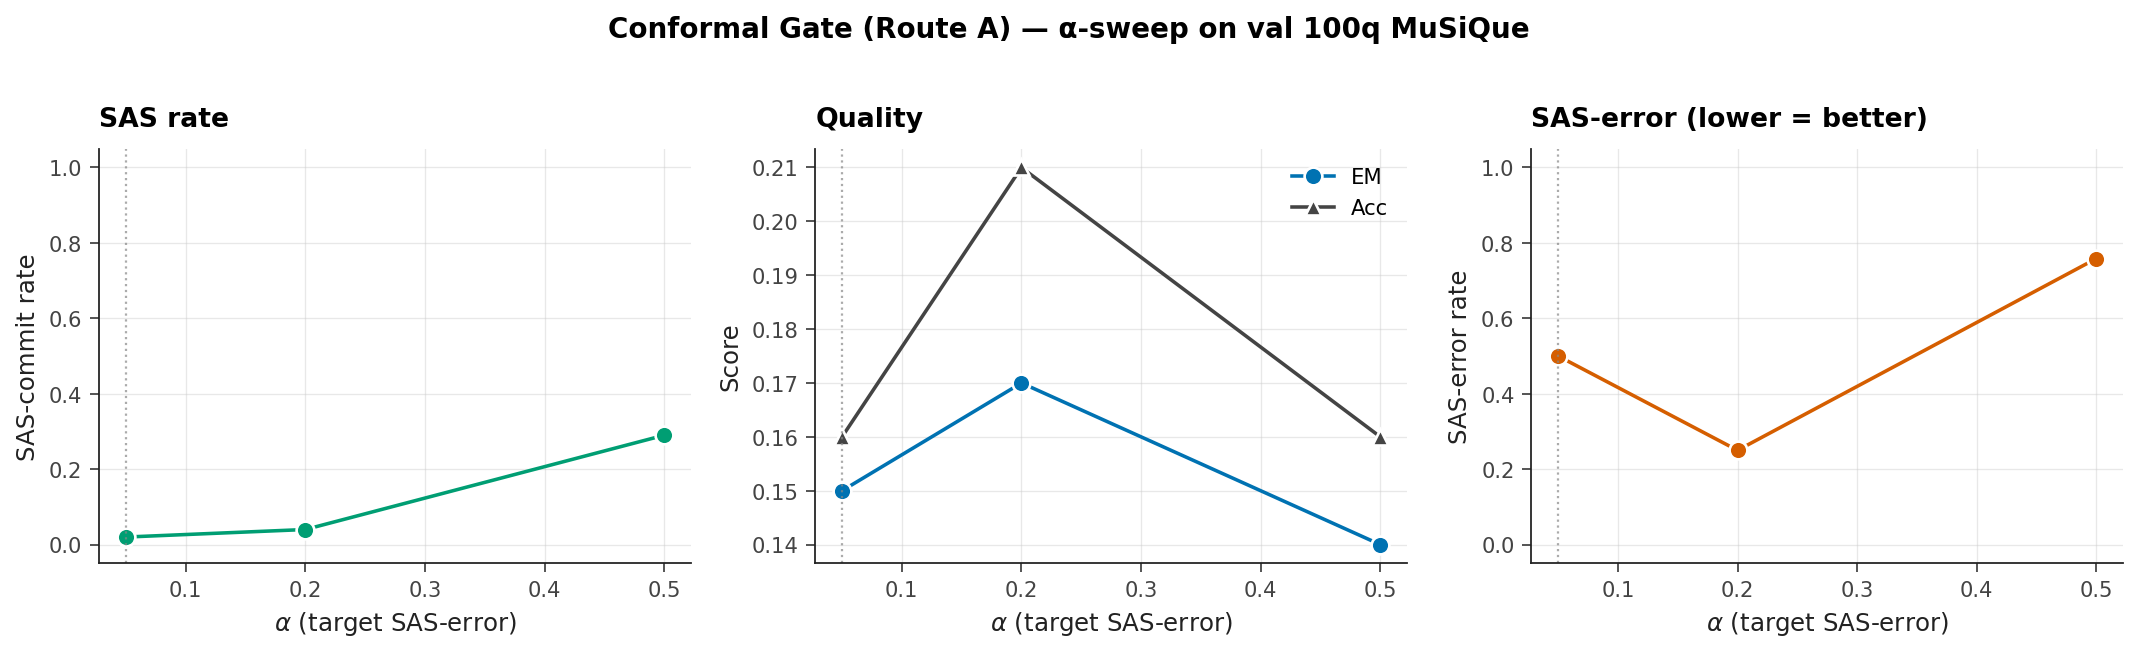
\includegraphics[width=0.85\linewidth]{figs/alpha_sweep.png}
\caption{Conformal gate $\alpha$-sweep on the 200q calibration pool.}
\label{fig:alphasweep}
\end{figure}

\subsubsection{Bayesian gate (Route B): $\tau_b$ and $\lambda$ sweeps}
\label{sec:bayes-results}

Tables~\ref{tab:taub} and~\ref{tab:lambda} report the two parameter sweeps
for the closed-system gate.

\begin{table}[H]
\centering
\small
\begin{tabular}{rrrrrr}
\toprule
$\tau_b$ & SAS rate & EM & F1 & Acc & avg tokens \\
\midrule
0.7 & \phantom{0}99\% & 0.085 & 0.161 & 0.115 & \phantom{0}\phantom{0}922 \\
0.9 & \phantom{0}94\% & 0.110 & 0.170 & 0.130 & 1\,395 \\
1.0 & \phantom{0}\phantom{0}2\% & 0.140 & 0.207 & 0.165 & 9\,418 \\
1.1 & \phantom{0}\phantom{0}0\% & 0.130 & 0.207 & 0.165 & 9\,559 \\
1.2 & \phantom{0}\phantom{0}0\% & 0.135 & 0.211 & 0.170 & 9\,475 \\
1.3 & \phantom{0}\phantom{0}0\% & 0.120 & 0.198 & 0.155 & 9\,569 \\
\bottomrule
\end{tabular}
\caption{Route B v2 $\tau_b$-sweep (200q val slice from MuSiQue, $\lambda$
fixed). The gate is bimodal: it commits on essentially every question for
$\tau_b \leq 0.9$ and on essentially none for $\tau_b \geq 1.0$.}
\label{tab:taub}
\end{table}

\begin{table}[H]
\centering
\small
\begin{tabular}{rrrrrr}
\toprule
$\lambda$ & SAS rate & EM & F1 & Acc & avg tokens \\
\midrule
$1\!\times\!10^{-5}$ & 100.0\% & 0.090 & 0.166 & 0.125 & 840 \\
$5\!\times\!10^{-5}$ & 100.0\% & 0.095 & 0.163 & 0.115 & 840 \\
$1\!\times\!10^{-4}$ & 100.0\% & 0.090 & 0.155 & 0.110 & 840 \\
$3\!\times\!10^{-4}$ & 100.0\% & 0.090 & 0.156 & 0.115 & 840 \\
$1\!\times\!10^{-3}$ & \phantom{0}99.5\% & 0.090 & 0.159 & 0.115 & 886 \\
$3\!\times\!10^{-3}$ & 100.0\% & 0.090 & 0.155 & 0.115 & 840 \\
\bottomrule
\end{tabular}
\caption{Route B v1 (entropy-only) $\lambda$-sweep over five orders of
magnitude on the same 200q val slice. The gate commits on essentially
every question regardless of $\lambda$ because the belief entropy is
zero at probe group size $G=1$.}
\label{tab:lambda}
\end{table}

The two sweeps confirm the negative-baseline reading of the closed-system
gate. Route~B v1 is degenerate by construction at $G=1$
(Eq.~\ref{eq:bayes-v1}). Route~B v2 (Eq.~\ref{eq:bayes-v2}) is bimodal:
the threshold either includes every probe ($\tau_b \leq 0.9$) or excludes
every probe ($\tau_b \geq 1.0$). There is no useful intermediate
operating point on this val slice. The flip happens because the
top-candidate net-score distribution at $G=1$ is concentrated very near
1.0, so any $\tau_b$ inside the concentration region either passes all or
none.

The headline result is therefore that the foreign-verifier path
(Route~A) is the only operating point that produces a graded, calibrated
SAS rate. This is the empirical justification for the conformal-gate
design choice.

\begin{figure}[H]
\centering
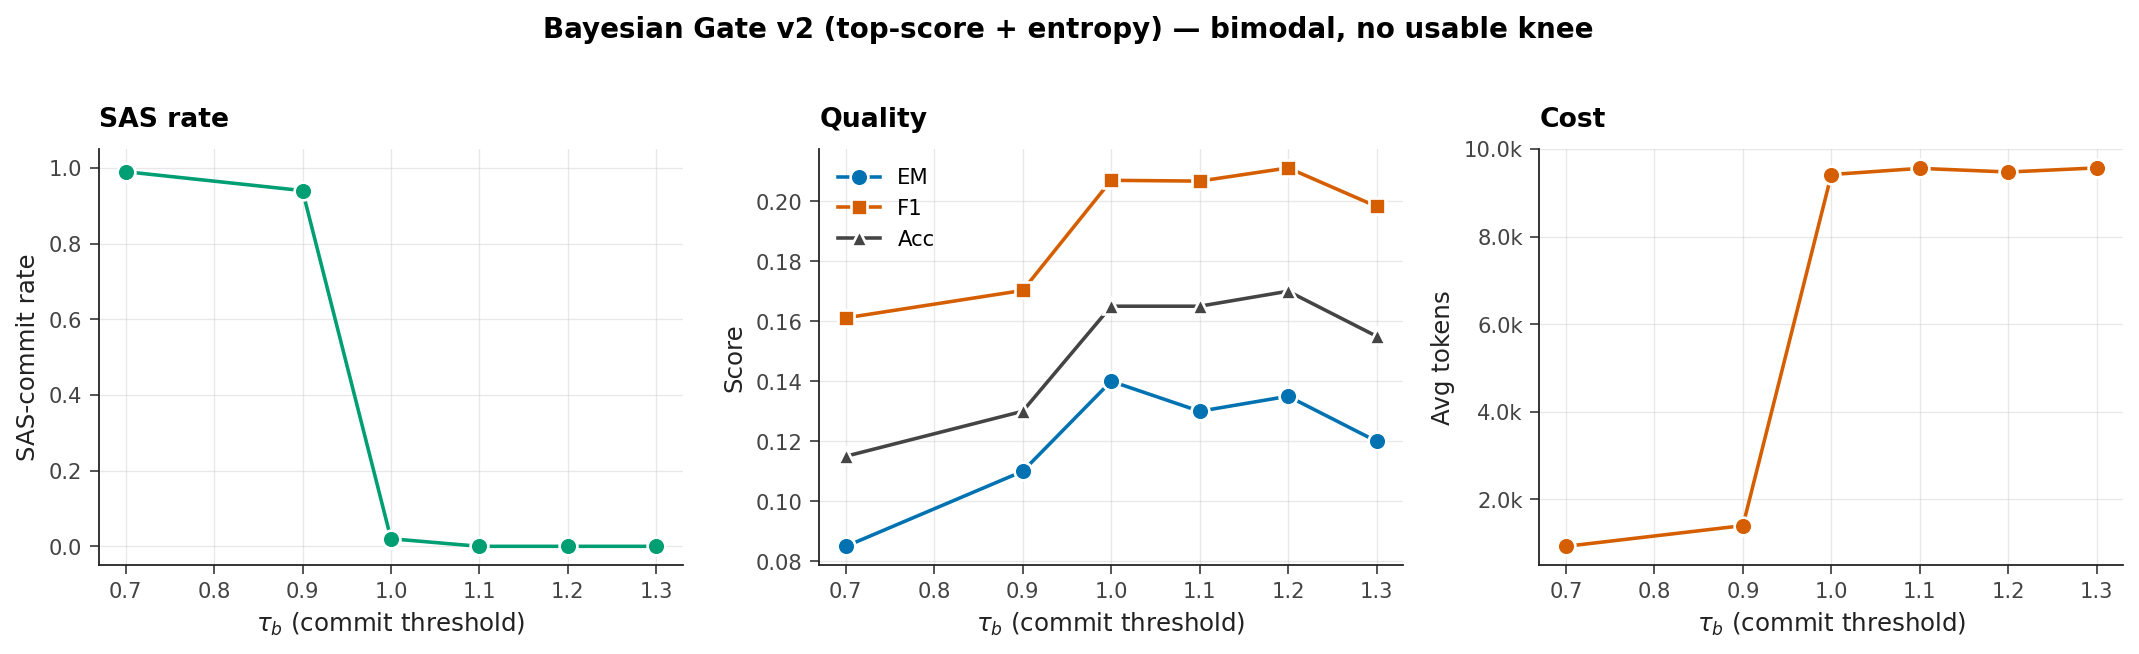
\includegraphics[width=0.92\linewidth]{figs/tau_b_sweep_v2.png}
\caption{Route B v2 $\tau_b$-sweep (200q MuSiQue val). The gate is bimodal:
$\tau_b\!\leq\!0.9$ commits $\approx$100\% of probes; $\tau_b\!\geq\!1.0$
commits $\approx$0\%. There is no useful intermediate operating point.}
\label{fig:taub}
\end{figure}

\begin{figure}[H]
\centering
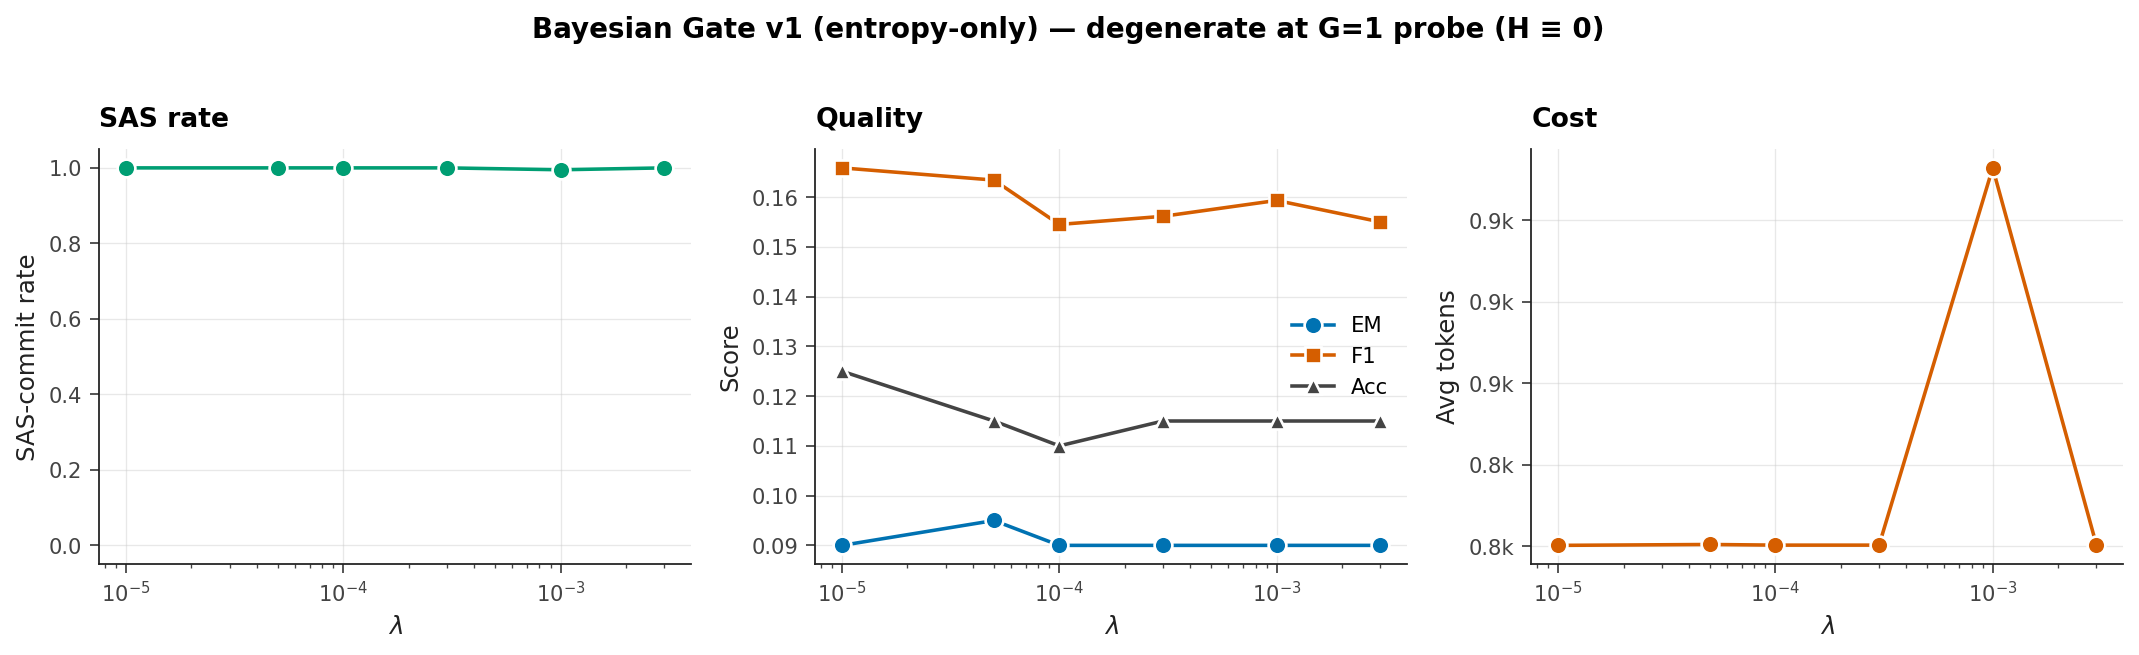
\includegraphics[width=0.92\linewidth]{figs/lambda_sweep.png}
\caption{Route B v1 $\lambda$-sweep over five orders of magnitude on the
200q MuSiQue val slice. The gate is degenerate at $G\!=\!1$: belief
entropy is zero by construction with a single probe sample, so the
entropy-only commit rule fires for every $\lambda$.}
\label{fig:lambda}
\end{figure}

\subsubsection{Headline view: where Route~B sits on the Pareto curves}

On the four 1000-question test sets the closed-system gate
(\amas-bayesian) is locked at the operating point $\tau_b=0.7$ that
matches the v2 commit-everything regime. This produces token counts under
1\,000 per question but at substantial F1 cost. Across all four datasets,
\amas-bayesian sits below \amas-conformal on F1 by 6 to 10 percentage
points and below \hera-repro on F1 by 2 to 4pp. Its position on the
Pareto plots in Figure~\ref{fig:pareto} is therefore the high-token-saving,
low-quality corner that bounds the cost--quality tradeoff from below.

\subsection{Per-profile breakdown}

Each test question is annotated with a query profile (\texttt{bridge},
\texttt{comparison}, \texttt{intersection}, \texttt{temporal},
\texttt{causal}, \texttt{verification}, or \texttt{ambiguous}). Bridge is
the dominant profile in MuSiQue (96\%), so dataset-level numbers track the
bridge sub-population. Figure~\ref{fig:heatmap} shows the per-profile
breakdown on MuSiQue.

\begin{figure}[H]
\centering
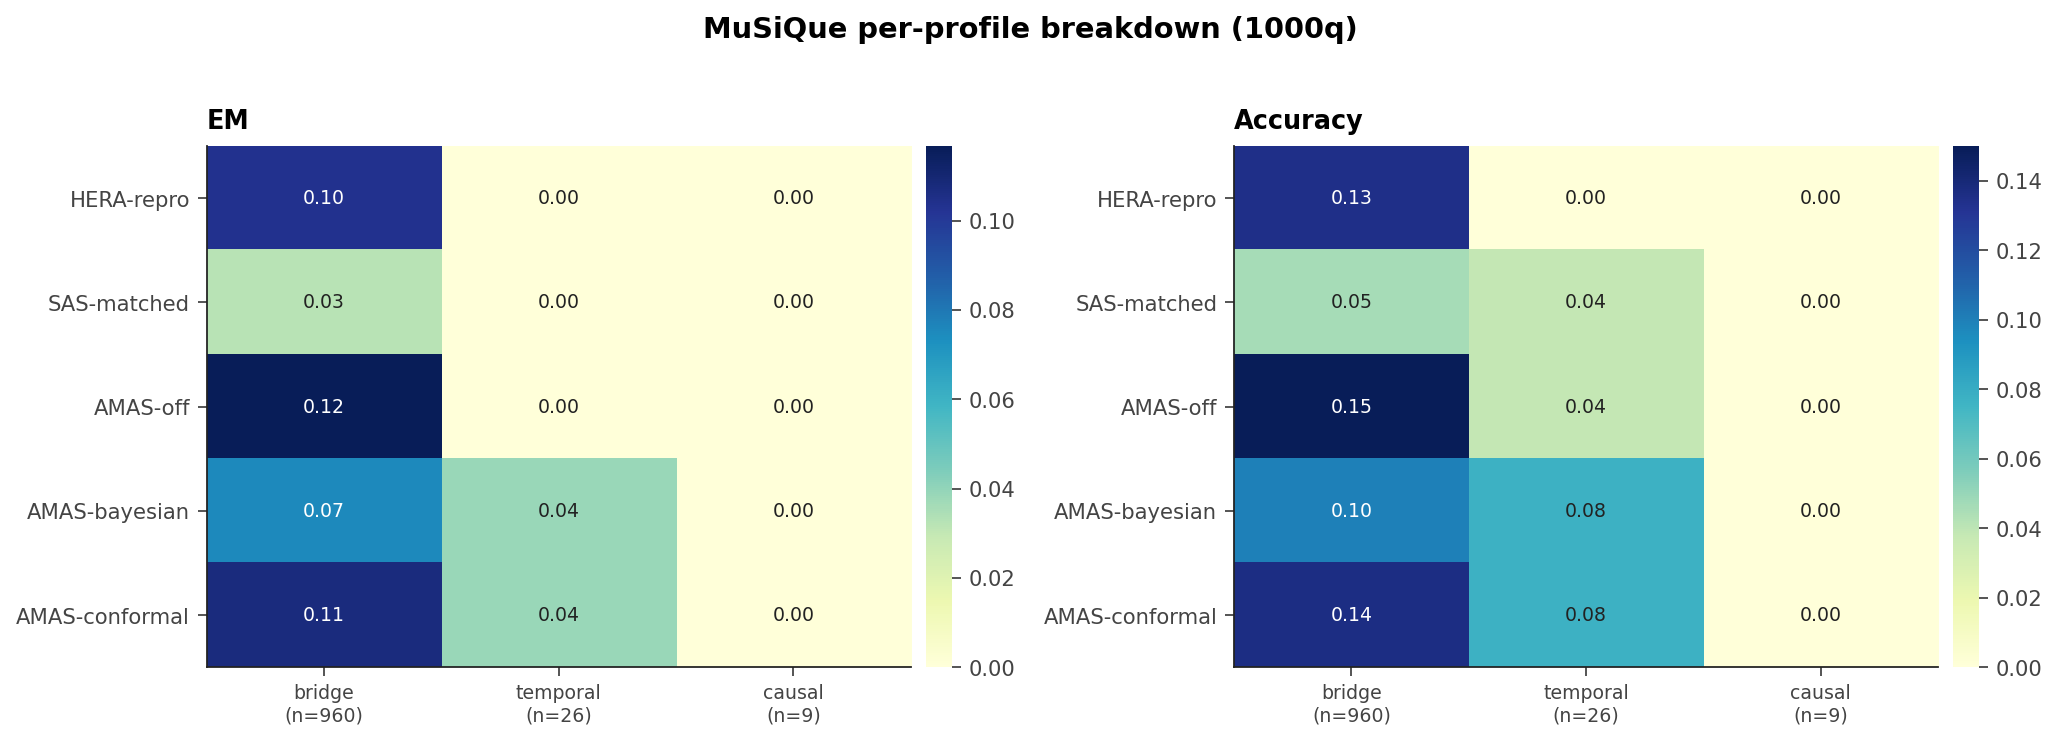
\includegraphics[width=0.85\linewidth]{figs/profile_heatmap_musique.png}
\caption{Per-profile EM/Acc heatmap on MuSiQue (n=1000). Bridge dominates.}
\label{fig:heatmap}
\end{figure}

\section{Limitations and future work}

\paragraph{Probe contamination.}
The probe and the verifier are both \code{gpt-4o-mini}, whose pre-training
corpus contains Wikipedia. Probe answers may therefore reflect memorization
rather than retrieval. \hera-repro shares the same property (its
sub-agents are also \code{gpt-4o-mini}), so the comparison is symmetric, but
a closed-book \code{gpt-4o-mini} ablation on the same 1000-question
evaluation is required to isolate the contribution of retrieval. This is
left for the next iteration.

\paragraph{Cross-family probe.}
A cross-family probe (e.g., Qwen3-14B for the probe with \code{gpt-4o-mini}
verifier) would weaken the contamination critique by breaking pre-training
correlation. We tried this configuration in an earlier iteration and
observed that the conformal commit rate collapsed from $40$--$66\%$ to
$0.3$--$7.9\%$, primarily because the verifier scored Qwen-style outputs
more harshly. Bringing back the cross-family probe will require either
re-training the verifier or relaxing the verifier's scoring rubric.

\paragraph{Stronger \hera baseline.}
The \hera-repro baseline used here corresponds to the published \hera
evaluation at the same compute level. A separately RoPE-trained \hera
checkpoint exists (\code{run02}) and reaches higher F1 at lower token cost.
\amas without TF-GRPO+RoPE training does not consistently match
RoPE-trained \hera; pursuing \amas-side training is the next step.

\paragraph{Adaptive depth.}
The current pipeline runs $T_{\max}=1$ \mas turn after the probe. A natural
extension is to make the depth adaptive --- run a second \mas turn only
when the verifier remains uncertain after turn~1. The conformal gate
already supports a turn-level \texttt{STOP} action; running it inside a
$T_{\max}=2$ pipeline is straightforward and is left for the next
iteration.

\paragraph{Lane-aware library.}
The experience library is currently lane-agnostic. Tagging insights with the
lane they were learned on (\sas vs \mas) and filtering retrieval by lane is
a small change that should improve specialization.

\section{Conclusion}

\amas demonstrates that adaptive routing between a single-shot probe and a
multi-agent search lane, governed by a calibrated foreign verifier, is a
clean Pareto improvement over a matched-untrained \hera baseline on four
multi-hop QA benchmarks. The \sas-lane commit rate adapts to dataset
difficulty (40.5\%--66.4\%), and on HotpotQA and Bamboogle the verifier
correctly routes easier questions to the cheap lane: mean \sas-committed
F1 exceeds the F1 of the questions handed to \mas. The token saving ranges
from 30\% to 55\% across datasets at matched-or-better quality. The
conformal gate has a marginal coverage guarantee at $\alpha=0.05$ and
calibrates on a 200-question pool that is id-disjoint from all evaluation
sets. The principal remaining limitation is that the \mas lane is not yet
trained on \amas-side data; with TF-GRPO+RoPE training on the \amas
pipeline we expect further token reduction at parity quality.

\paragraph{Code and data.}
The system as evaluated here is at commit \code{e54070389} of the
\code{adaptive-mas/amas} repository. Calibration data, predictions,
summaries, plot sources, and per-question \sas-correctness rolls live under
\code{results/p1\_full/} and \code{reports/v1/}.

\begin{thebibliography}{9}
\bibitem{hera-paper}
HERA: Hierarchical Experience Replay for Adaptive Multi-agent RAG.
Reference reproduction at \url{reproduction/hera/}.
\bibitem{conformal-prediction}
Vovk, Gammerman, Shafer. \emph{Algorithmic Learning in a Random World}.
Springer 2005.
\bibitem{tran-kiela}
Tran and Kiela. ``On the Necessity of Multi-Agent Architectures for RAG.''
Single-agent retrieve-then-answer baseline used as the lower-bound
reference (\textit{SAS-matched}).
\bibitem{musique}
Trivedi et al. ``MuSiQue: Multihop Questions via Single-hop Question
Composition.'' \emph{TACL} 2022.
\bibitem{hotpot}
Yang et al. ``HotpotQA: A Dataset for Diverse, Explainable Multi-hop
Question Answering.'' \emph{EMNLP} 2018.
\bibitem{2wiki}
Ho et al. ``Constructing A Multi-hop QA Dataset for Comprehensive
Evaluation of Reasoning Steps.'' \emph{COLING} 2020.
\bibitem{bamboogle}
Press et al. ``Measuring and Narrowing the Compositionality Gap in
Language Models.'' Bamboogle dataset.
\end{thebibliography}

\end{document}
